% =====================================================================================================
% BASIC OUTLINE of the multimodal paper.
%
% Language: ASD-STE100 Simplified Technical English. Rules used in this file:
%   - One topic in each sentence. Descriptive sentences have 25 words or fewer.
%   - Active voice. Simple tenses. No noun clusters of more than three words.
%   - Approved words where possible (for example "use", not "utilize"; "show", not "demonstrate").
%   - Technical names (RS, LOO, PSNR, JSCC) are technical nouns and stay as they are.
%
% Format: section layout of the ADJSCC paper (Xu et al., "Wireless Image Transmission Using Deep Source
% Channel Coding With Attention Modules", IEEE TCSVT 2022): Introduction, Related Work, System Model,
% Proposed Method (architecture figure, then one module per subsection), Experimental Results (setup,
% performance, ablation, analysis, complexity and storage), Conclusion.
%
% The full prose draft with every table is in main_detailed_draft.tex. The source of each number is in
% RESULTS_COMPENDIUM.md. Items in red (\TBD) are open.
% =====================================================================================================
\documentclass[journal]{IEEEtran}
\usepackage{amsmath,amssymb,amsthm}
\usepackage{graphicx}
\usepackage{booktabs}
\usepackage{xcolor}
\usepackage{cite}
\usepackage{url}
\usepackage{pifont}
\usepackage{tikz}
\usetikzlibrary{positioning,arrows.meta,calc}

\newtheorem{lemma}{Lemma}
\newtheorem{proposition}{Proposition}
\providecommand{\TBD}[1]{\textbf{\color{red}[#1]}}

\graphicspath{{../results/}{../published_results/}{../paper/figures/}{figures/}}
\newcommand{\figbox}[2]{%
  \fbox{\parbox[c][3.2cm][c]{\dimexpr#1-2\fboxsep-2\fboxrule\relax}{\centering\footnotesize\color{gray}\textbf{FIGURE TO MAKE}\\[2pt]#2}}}
\newcommand{\resfig}[3]{%
  \IfFileExists{../results/#2}{\includegraphics[width=#1]{#2}}{%
  \IfFileExists{../published_results/#2}{\includegraphics[width=#1]{#2}}{%
  \IfFileExists{../paper/figures/#2}{\includegraphics[width=#1]{#2}}{\figbox{#1}{#3\\(\texttt{#2})}}}}}

\begin{document}

\title{Which Latent Bytes Need Parity? Importance-Aware Reed--Solomon Protection of Deep JSCC Latents
for Images, Speech and Text over Packet-Erasure Channels}
\author{\TBD{Authors}}
\maketitle

% -----------------------------------------------------------------------------------------------------
\begin{abstract}
% Outline of the abstract. One sentence for each point.
\begin{itemize}
\item Deep JSCC sends a learned latent. Packet networks lose full packets.
\item We quantize the latent to bytes and protect the bytes with Reed--Solomon (RS) codes.
\item The question: which latent bytes must get the parity when the parity budget is fixed?
\item We use one latent format for images, speech and text: 16 channels of 64 bytes in 96 packets.
\item We measure the damage when one latent channel is lost (leave-one-out, LOO).
\item The damage is not equal. Four of 16 channels cause 33--53\% of the damage for images and speech.
\item For text, the damage is almost equal (28--30\%; 25\% is fully equal).
\item Attention gates do not show which channels are important. Latent energy and a small head do.
\item The best use of the parity at a known loss rate is truncation: send only the important channels,
      with one strong code.
\item At 40\% packet loss, truncation gives 6.5~dB more than equal protection for images.
\item Three-tier protection gives 1.5--3.4~dB for speech. For text, it gives no useful gain.
\end{itemize}
\end{abstract}

\begin{IEEEkeywords}
Deep joint source-channel coding, unequal error protection, Reed--Solomon codes, packet erasure channel,
speech transmission, text transmission.
\end{IEEEkeywords}

% =====================================================================================================
\section{Introduction}
% ADJSCC format: problem -> limit of current methods -> our method -> contributions -> paper layout.
\subsection*{Problem}
\begin{itemize}
\item Deep JSCC maps a source directly to channel symbols with one neural network.
\item The quality of deep JSCC decreases slowly when the channel becomes worse \cite{bourtsoulatze2019deep}.
\item Most deep JSCC studies use a noise channel or a fading channel.
\item Many real links send bytes in packets. A network loses full packets.
\item The receiver knows which packets are lost. This is an erasure channel.
\end{itemize}
\subsection*{Limits of current methods}
\begin{itemize}
\item Reed--Solomon (RS) codes correct erasures. An RS$(n,k)$ code recovers its data from any $k$ of its $n$ symbols.
\item Classical unequal protection needs a known order of importance in the bit stream \cite{albanese1996pet,mohr2000ulp}.
\item A JSCC latent has no known order.
\item Prior work uses attention weights as importance \cite{uyanik2023gradfec,zhan2026isfr}. Nobody tested this for packet loss.
\end{itemize}
\subsection*{Our method}
\begin{itemize}
\item We quantize the latent to bytes. One latent value is one byte and one RS symbol.
\item We measure the importance of each latent channel.
\item We give more parity to important channels, or we do not send unimportant channels.
\item We use the same method for images, speech and text.
\end{itemize}
\subsection*{Contributions}
\begin{enumerate}
\item One byte interface and one RS pipeline for three modalities (Fig.~\ref{fig:workflow}).
\item A measurement of erasure sensitivity in each modality, with and without attention modules.
\item Proof that attention gates do not predict erasure damage. Simple predictors that do.
\item An exact model of RS decoding and an optimal parity allocation.
\item Rules, set before the test, that tell when unequal protection is useful.
\end{enumerate}
\subsection*{Paper layout}
\begin{itemize}
\item Section~\ref{sec:related} gives related work. Section~\ref{sec:model} gives the system model.
\item Section~\ref{sec:method} gives the method. Section~\ref{sec:exp} gives the results.
\item Section~\ref{sec:conclusion} gives the conclusion.
\end{itemize}

% =====================================================================================================
\section{Related Work}\label{sec:related}
% ADJSCC format: two or three short subsections.
\subsection{Deep JSCC}
\begin{itemize}
\item Deep JSCC for images \cite{bourtsoulatze2019deep}. Bandwidth-agile deep JSCC \cite{kurka2021bandwidth}.
\item ADJSCC adds attention modules that change each channel with the SNR \cite{xu2022adjscc}.
\item DeepJSCC-Q quantizes the latent for digital links \cite{tung2022deepjsccq}.
\item Learned latents over packet loss \cite{esfahanizadeh2026block,bo2026lgsemcom,wei2026everypacket}.
\item Semantic communication for text and speech \cite{xie2021deepsc,weng2021deepscs}. \TBD{Add speech and text under packet loss.}
\end{itemize}
\subsection{Unequal error protection}
\begin{itemize}
\item PET codes each priority class over all packets \cite{albanese1996pet}.
\item ULP and optimal packetization protect an embedded bit stream \cite{mohr2000ulp,dumitrescu2004optimal,hamzaoui2005optimized}.
\item These methods need a known order. A JSCC latent does not have one.
\end{itemize}
\subsection{Importance of learned features}
\begin{itemize}
\item Grad-FEC ranks feature packets with Grad-CAM \cite{uyanik2023gradfec}. ISFR uses the LOO drop \cite{zhan2026isfr}.
\item Attention weights often do not predict ablation damage \cite{jain2019attention,morcos2018single}.
\item Nested dropout puts an order into a latent during training \cite{rippel2014nested}.
\end{itemize}

% =====================================================================================================
\section{System Model}\label{sec:model}
% ADJSCC format: one block diagram, then the variables and the problem.
\begin{figure}[t]\centering
\resizebox{\columnwidth}{!}{%
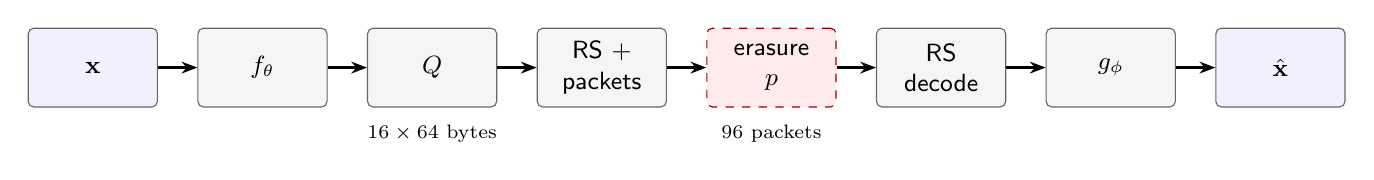
\begin{tikzpicture}[font=\sffamily\small, >={Stealth[length=2mm]}, node distance=4mm and 5mm,
  b/.style={draw=black!60, fill=black!4, rounded corners=2pt, align=center, minimum height=10mm, text width=15mm, inner sep=2pt},
  c/.style={b, fill=red!8, draw=red!60!black, dashed}]
\node[b, fill=blue!6] (x) {$\mathbf{x}$};
\node[b, right=of x] (f) {$f_\theta$};
\node[b, right=of f] (q) {$Q$};
\node[b, right=of q] (e) {RS +\\packets};
\node[c, right=of e] (ch) {erasure\\$p$};
\node[b, right=of ch] (d) {RS\\decode};
\node[b, right=of d] (g) {$g_\phi$};
\node[b, fill=blue!6, right=of g] (xh) {$\hat{\mathbf{x}}$};
\foreach \a/\b in {x/f,f/q,q/e,e/ch,ch/d,d/g,g/xh} \draw[->, thick] (\a) -- (\b);
\node[below=1mm of q, font=\scriptsize] {$16\times64$ bytes};
\node[below=1mm of ch, font=\scriptsize] {96 packets};
\end{tikzpicture}}
\caption{System model.}\label{fig:system}
\end{figure}
\begin{itemize}
\item The encoder $f_\theta$ maps a source $\mathbf{x}$ to a latent of 16 channels with 64 values each.
\item The quantizer $Q$ changes each value to one byte. The latent has 1,024 bytes.
\item The transmitter sends 96 packets of 16 bytes. This gives 50\% parity.
\item The channel erases each packet with probability $p$. The receiver knows the lost packets.
\item The RS decoder recovers lost bytes if possible. It sets the other lost bytes to zero.
\item The decoder $g_\phi$ makes the output $\hat{\mathbf{x}}$.
\item Problem: find the channel order $\pi$ and the code layout that give the smallest expected distortion.
      The total number of packets is fixed at 96.
\end{itemize}
\begin{table}[t]\centering\caption{Sources and the shared latent format}\label{tab:modalities}
\resizebox{\columnwidth}{!}{%
\begin{tabular}{llll}\toprule
 & Image & Speech & Text\\\midrule
Dataset & CIFAR-10 & LibriSpeech & text8\\
Sample & $32\times32$ image & 1.024~s segment & 2,048 characters\\
Latent & \multicolumn{3}{c}{16 channels $\times$ 64 bytes}\\
Metric & PSNR (dB) & SNR (dB) & character accuracy (\%)\\
\bottomrule\end{tabular}}
\end{table}

% =====================================================================================================
\section{Proposed Method}\label{sec:method}
% ADJSCC format: the full architecture figure first, then one subsection for each module.
\subsection{Architecture}
\begin{figure*}[t]\centering
\resizebox{\textwidth}{!}{%
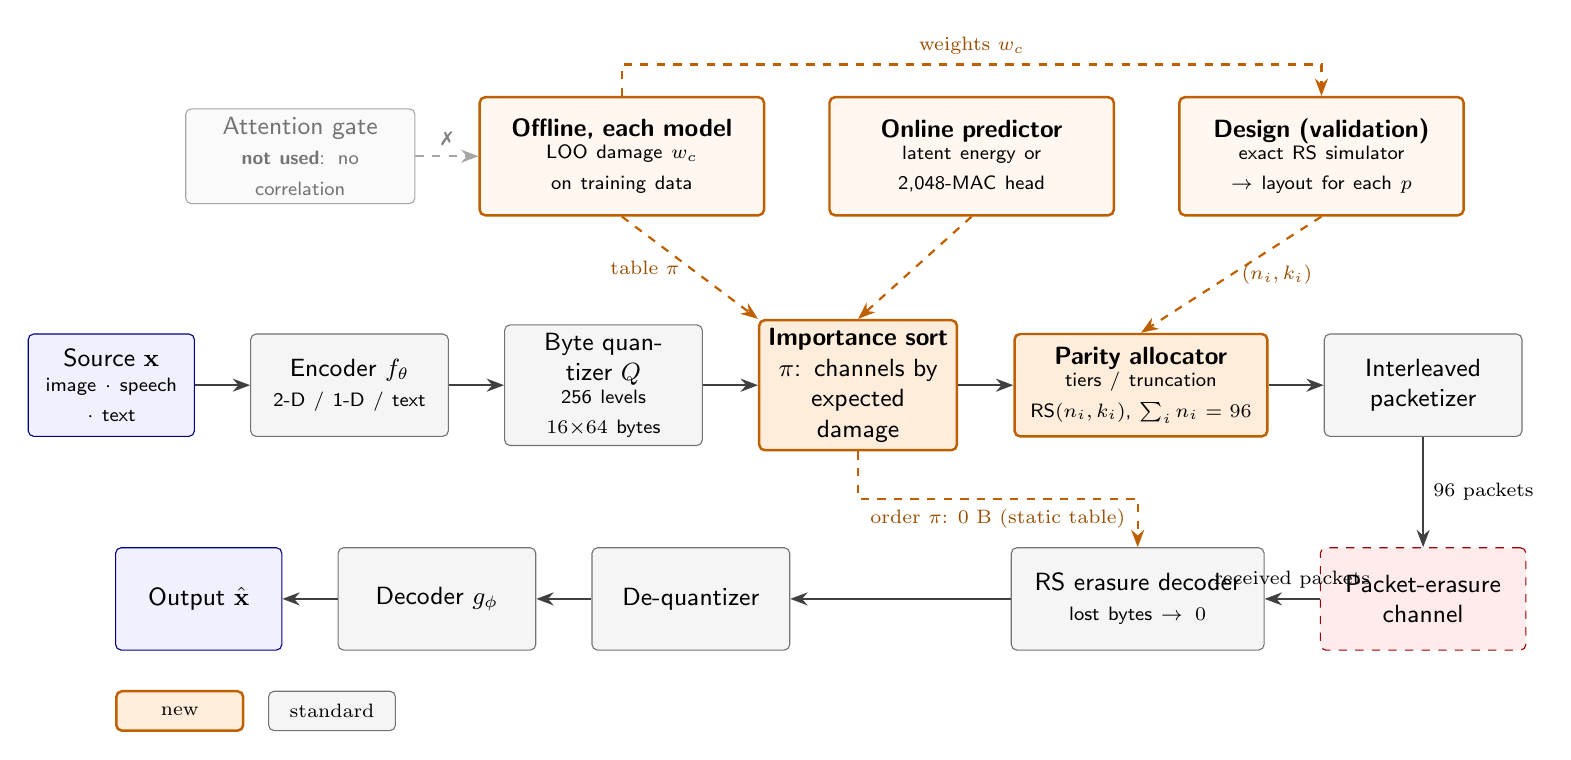
\begin{tikzpicture}[
  font=\sffamily\small, >={Stealth[length=2.2mm]}, node distance=6mm and 7mm,
  std/.style={draw=black!55, fill=black!4, rounded corners=2pt, align=center, minimum height=13mm,
              text width=23mm, inner sep=3pt},
  new/.style={std, draw=orange!75!black, fill=orange!14, line width=0.9pt},
  src/.style={std, text width=19mm, fill=blue!6, draw=blue!50!black},
  chan/.style={std, fill=red!8, draw=red!60!black, dashed, text width=24mm},
  off/.style={new, fill=orange!6, text width=34mm, minimum height=15mm},
  bad/.style={std, fill=black!2, draw=black!35, text=black!55, text width=27mm, minimum height=10mm},
  flow/.style={->, line width=0.8pt, draw=black!75},
  side/.style={->, line width=0.8pt, draw=orange!75!black, dashed}]
\node[src] (x) {Source $\mathbf{x}$\\[1pt]\scriptsize image $\cdot$ speech\\\scriptsize $\cdot$ text};
\node[std, right=of x] (enc) {Encoder $f_\theta$\\\scriptsize 2-D / 1-D / text};
\node[std, right=of enc] (q) {Byte quantizer $Q$\\\scriptsize 256 levels\\\scriptsize $16{\times}64$ bytes};
\node[new, right=of q] (sort) {\textbf{Importance sort}\\$\pi$: channels by\\expected damage};
\node[new, right=of sort, text width=30mm] (alloc) {\textbf{Parity allocator}\\\scriptsize tiers / truncation\\\scriptsize RS$(n_i,k_i)$, $\sum_i n_i = 96$};
\node[std, right=of alloc] (pkt) {Interleaved\\packetizer};
\node[chan, below=14mm of pkt] (ch) {Packet-erasure\\channel};
\node[std, left=of ch, text width=30mm] (rsdec) {RS erasure decoder\\\scriptsize lost bytes $\to 0$};
\node[std, left=of rsdec, xshift=-21mm] (deq) {De-quantizer};
\node[std, left=of deq] (dec) {Decoder $g_\phi$};
\node[src, left=of dec] (xh) {Output $\hat{\mathbf{x}}$};
\node[off, above=13mm of sort, xshift=-30mm] (loo) {\textbf{Offline, each model}\\\scriptsize LOO damage $w_c$\\\scriptsize on training data};
\node[off, right=8mm of loo] (proxy) {\textbf{Online predictor}\\\scriptsize latent energy or\\\scriptsize 2,048-MAC head};
\node[off, right=8mm of proxy] (sim) {\textbf{Design (validation)}\\\scriptsize exact RS simulator\\\scriptsize $\to$ layout for each $p$};
\node[bad, left=8mm of loo] (att) {Attention gate\\\scriptsize \textbf{not used}: no correlation};
\draw[flow] (x) -- (enc); \draw[flow] (enc) -- (q); \draw[flow] (q) -- (sort);
\draw[flow] (sort) -- (alloc); \draw[flow] (alloc) -- (pkt);
\draw[flow] (pkt) -- node[right, font=\scriptsize] {96 packets} (ch);
\draw[flow] (ch) -- node[above, font=\scriptsize] {received packets} (rsdec);
\draw[flow] (rsdec) -- (deq); \draw[flow] (deq) -- (dec); \draw[flow] (dec) -- (xh);
\draw[side] (loo.south) -- node[left, font=\scriptsize, text=orange!60!black] {table $\pi$} (sort.north west);
\draw[side] (proxy.south) -- (sort.north);
\draw[side] (sim.south) -- node[right, font=\scriptsize, text=orange!60!black] {$(n_i,k_i)$} (alloc.north);
\draw[side] (loo.north) |- ++(0,4mm) -| node[pos=0.25, above, font=\scriptsize, text=orange!60!black] {weights $w_c$} (sim.north);
\draw[->, line width=0.8pt, draw=black!35, dashed] (att.east) -- node[above, font=\scriptsize, text=black!50] {\ding{55}} (loo.west);
\draw[side] (sort.south) -- ++(0,-6mm) -| node[pos=0.25, below, font=\scriptsize, text=orange!60!black]
      {order $\pi$: 0 B (static table)} (rsdec.north);
\node[new, text width=14mm, minimum height=5mm, below=5mm of xh.south west, anchor=north west, font=\scriptsize] (l1) {new};
\node[std, text width=14mm, minimum height=5mm, right=3mm of l1, font=\scriptsize] (l2) {standard};
\end{tikzpicture}}
\caption{Proposed pipeline. Orange blocks are new in this work. Grey blocks are standard deep JSCC.}
\label{fig:workflow}
\end{figure*}
\begin{itemize}
\item Fig.~\ref{fig:workflow} shows the full pipeline.
\item The grey blocks are a standard quantized deep JSCC.
\item The orange blocks are new: the importance sort, the parity allocator and their design tools.
\item The same pipeline is used for images, speech and text. Only the encoder and decoder change.
\end{itemize}

\subsection{Encoder, decoder and attention modules}
\begin{itemize}
\item ADJSCC-Q: the ADJSCC network \cite{xu2022adjscc} with an attention module after each layer.
\item DeepJSCC-Q: the same network without attention modules.
\item Images use 2-D convolutions. Speech and text use 1-D convolutions.
\item We train both types for each modality. This gives an attention ablation in each modality.
\end{itemize}

\subsection{Byte quantizer}
\begin{itemize}
\item The quantizer has 256 learned levels. One latent value becomes one byte.
\item Training uses a soft-to-hard method, as in DeepJSCC-Q \cite{tung2022deepjsccq}.
\item The quantizer decreases the clean PSNR by approximately 0.5~dB for images.
\end{itemize}

\subsection{Erasure sensitivity}
\begin{itemize}
\item We erase one latent channel (64 bytes) and decode. We record the quality drop.
\item We do this for each of the 16 channels on the training data. This gives the LOO damage $w_c$.
\item We sort the channels by $w_c$. This gives a static order $\pi$ for each model.
\item The decoder keeps the same table. Thus the order needs no side information.
\item \TBD{Use one definition of ``top-4 share'' for all modalities (dB share or MSE share).}
\end{itemize}

\subsection{Importance predictors}
\begin{itemize}
\item Static table: the training-data order of the model.
\item Latent energy, $\ell_1$ norm, variance and Taylor saliency of each channel.
\item A small head: a two-layer network with 2,048 multiply-accumulate operations.
\item The attention gate of the bottleneck module. This is the prior-work baseline.
\item We score each predictor against the true damage of each sample.
\end{itemize}

\subsection{Exact RS outcome and parity allocation}
\begin{lemma}
A data byte is lost if its packet is lost and its codeword has more than $n-k$ lost symbols.
Thus a byte of an RS$(n,k)$ code is lost with probability $q(n,k,p)=p\,\Pr[\mathrm{Bin}(n-1,p)\ge n-k]$.
\end{lemma}
\begin{itemize}
\item The lemma replaces the RS decoder in simulation. The result is exact.
\item An additive model of the distortion uses $w_c$ and $q(n,k,p)$.
\item Dynamic programming finds the best layout for this model.
\item The exact simulator checks the best layouts on validation data.
\end{itemize}
\begin{proposition}
Truncation to the top $m$ channels is better than equal protection if the lost damage of the
$16-m$ channels that are not sent is less than the protection that the extra parity gives.
\end{proposition}
\begin{itemize}
\item Thus truncation needs a correct order. A random order removes important channels.
\end{itemize}

\subsection{Packet layouts}
\begin{figure}[t]\centering
\figbox{\columnwidth}{Packet layouts: interleaved RS(96,64); three tiers RS(32,16), RS(48,32), (16,16);
truncation RS($96,4m$).}
\caption{Packet layouts with the same 96 packets.}\label{fig:layout}
\end{figure}
\begin{itemize}
\item Each packet carries one symbol of each codeword (interleaving). A lost packet costs each codeword one symbol.
\item Uniform: RS(96,64) on all channels. This is equal protection.
\item Three tiers (25/50/25): RS(32,16) on the top 25\%, RS(48,32) on the middle 50\%, no parity on the bottom 25\%.
\item Truncation: RS$(96,4m)$ on the top $m$ channels. The other channels are not sent.
\item Under burst loss, we interleave the packets of all tiers.
\end{itemize}

% =====================================================================================================
\section{Experimental Results}\label{sec:exp}
% ADJSCC format: setup, main performance, comparison, ablation, analysis, complexity.

\subsection{Experimental Setup}
\begin{itemize}
\item Images: CIFAR-10, 40k/10k/10k split. CIFAR-100 and Kodak for transfer tests.
\item Speech: LibriSpeech, 1.024~s segments. Text: text8, 2,048-character windows.
\item Seeds: 5 image ADJSCC-Q, 4 image DeepJSCC-Q, 3 + 3 speech, 2 text models converged.
\item A rule set before the test removes models that did not converge.
\item Five channel seeds. All methods use the same packet losses. Gains are paired.
\item Baselines: no RS, uniform RS, random order, attention order, PET, Grad-FEC style,
      smaller models, JPEG/JPEG2000/WebP with RS.
\item \TBD{Speech training loss; PESQ and STOI.}
\end{itemize}

\subsection{Performance on Images}
\begin{figure}[t]\centering
\resfig{\columnwidth}{fig_main.pdf}{PSNR vs loss, images}
\caption{PSNR versus packet loss rate, CIFAR-10.}\label{fig:img-main}
\end{figure}
\begin{itemize}
\item Uniform RS has no loss up to 20\%. It fails after 33\%: 20.73~dB at 40\% loss.
\item Three tiers give $+2.86$~dB at 40\% loss. They are worse below 32\% loss ($-0.95$~dB at 30\%).
\item Truncation gives $+6.52$~dB at 40\% loss (27.25~dB). It is never worse than uniform RS.
\item The best multi-tier layout is at most 0.15~dB better than truncation.
\item Across 8 image models, truncation gives $+4.0$ to $+9.4$~dB at 40\% loss.
\item A model with nested dropout keeps 30.60~dB at 40\% loss. Its clean cost is 0.24~dB.
\end{itemize}

\subsection{Performance on Speech}
\begin{figure}[t]\centering
\resfig{\columnwidth}{speech/deepjsccq1d/seed42/test_sweep/figures/test_sweep_psnr_curves.png}{SNR vs loss, speech}
\caption{Segment SNR versus packet loss rate, speech.}\label{fig:sp-main}
\end{figure}
\begin{itemize}
\item Four of 16 channels cause 43--46\% of the damage (family means).
\item Three tiers with LOO order give $+1.76$~dB (ADJSCC-Q-1D) and $+2.96$~dB (DeepJSCC-Q-1D) at 40\% loss.
\item A random order gives only $+0.81$ and $+0.63$~dB.
\item Both families pass the rules that we set before the test.
\item \TBD{Run truncation and the allocation search on speech.}
\end{itemize}

\subsection{Performance on Text}
\begin{figure}[t]\centering
\resfig{\columnwidth}{text/compare/sorted_profiles.png}{Sorted LOO damage, text}
\caption{Sorted LOO damage for text. The damage is almost equal in all channels.}\label{fig:tx-profiles}
\end{figure}
\begin{itemize}
\item Only 2 of 6 text models converged (69.2\% and 64.6\% clean character accuracy).
\item Four of 16 channels cause only 28--30\% of the damage. Each channel costs more than 12 points.
\item At 40\% loss, three tiers give $+2.57$ points. A random order gives $+1.74$ points.
\item At 40\% loss, all methods give 20--26\% accuracy. The text cannot be read.
\item At 30\% loss, three tiers are 12--17 points worse than uniform RS.
\item Result: for text, equal protection is the correct choice.
\end{itemize}

\subsection{Comparison with Other Methods}
\begin{itemize}
\item JPEG, JPEG2000 and WebP with fixed RS fail after 33\% loss (14--15~dB at 40\%).
\item WebP with a rate-adaptive RS code keeps 36.84~dB at 40\% loss. It is better than our JSCC models.
\item A 24-channel JSCC model without RS gives 24.36~dB at 40\%. RS with truncation gives 26.03~dB.
\item Grad-FEC-style drop-and-protect gives $+4.52$~dB at 40\% but costs 3.80~dB on a clean channel.
\end{itemize}

\subsection{Ablation Study}
\begin{table}[t]\centering\caption{Gain over uniform RS at 40\% loss for each channel order}\label{tab:ablation}
\resizebox{\columnwidth}{!}{%
\begin{tabular}{lccc}\toprule
Order & Image (tiers) & Image (truncation) & Speech ADJSCC-Q-1D (tiers)\\\midrule
LOO table & $+2.86$ & $+6.52$ & $+2.01$\\
Energy & $+2.92$ & $+6.00$ & $+2.10$\\
Head (2,048 MACs) & $+3.00$ & $+6.37$ & $+2.09$\\
Random & $+0.94$ & $+1.58$ & $+0.84$\\
Attention gate & $+0.74$ & $+4.80$ & $+0.37$\\
\bottomrule\end{tabular}}
\end{table}
\begin{itemize}
\item Same tiers, same packets: only the channel order changes (Table~\ref{tab:ablation}).
\item The order gives most of the gain. A random order recovers 23\% of it for images.
\item Without attention modules, the damage is also concentrated (33--40\% for images).
\item Two blocks of RS(48,32) without an order give $-0.05$~dB. Short blocks alone do not help.
\end{itemize}

\subsection{Analysis of Attention}
\begin{figure}[t]\centering
\resfig{0.49\columnwidth}{eval/oracle_attention_correlation.png}{Attention vs damage, images}\hfill
\resfig{0.49\columnwidth}{speech/adjsccq1d/seed42/attention/fig2_left_attention_scatter.png}{Attention vs damage, speech}
\caption{Attention gate value versus LOO damage: (a) images, (b) speech.}\label{fig:att}
\end{figure}
\begin{itemize}
\item In each sample, attention and damage have no correlation: $-0.015$ (images), $-0.22$ (speech), $-0.12$ (text).
\item The top four attention channels are not the top four damage channels (0.14--0.23; random gives 0.25).
\item Latent energy correlates well for images ($+0.84$) and speech ($+0.87$). It does not for text ($+0.42$).
\item The static table works for all modalities ($+0.77$ to $+0.89$, except ADJSCC-Q-1D: $+0.42$).
\item Attention modules make the latent more robust without RS. They do not show importance.
\end{itemize}

\subsection{Robustness}
\begin{itemize}
\item Bursts: tiers must be interleaved. At burst length 16, in-order tiers give $-0.56$~dB; interleaved give $+0.80$~dB.
\item Wrong loss rate: a layout for 40\% loss costs 2.59~dB on a clean channel. Use a selector.
\item Kodak images: three tiers give $+1.43$~dB at 40\% loss, with no penalty at low loss.
\item The CIFAR-10 order transfers to CIFAR-100 (Spearman 0.997).
\end{itemize}

\subsection{Complexity and Storage}
\begin{itemize}
\item Static table: 16 bytes in the decoder. No side information.
\item Head: 2,048 MACs. This is 0.039\% of the image encoder and 0.024\% of the speech encoder.
\item LOO table: 16 decoder passes for each training sample, one time for each model.
\item The receiver uses the same RS decoder as for uniform protection.
\end{itemize}

% =====================================================================================================
\section{Conclusion}\label{sec:conclusion}
\begin{itemize}
\item For images and speech, a small number of latent channels causes most of the erasure damage.
\item Attention gates do not find these channels. A static table, latent energy or a small head finds them.
\item At a known loss rate, truncation with one strong code is the best use of the parity.
\item The channel order gives most of the gain.
\item For text, the damage is almost equal. Equal protection is the correct choice.
\item Measure the importance first. Then decide if unequal protection is necessary.
\item Future work: entropy-coded latents, larger images, speech and text with truncation.
\end{itemize}

\bibliographystyle{IEEEtran}
\bibliography{../paper/references,references_extra}
\end{document}
